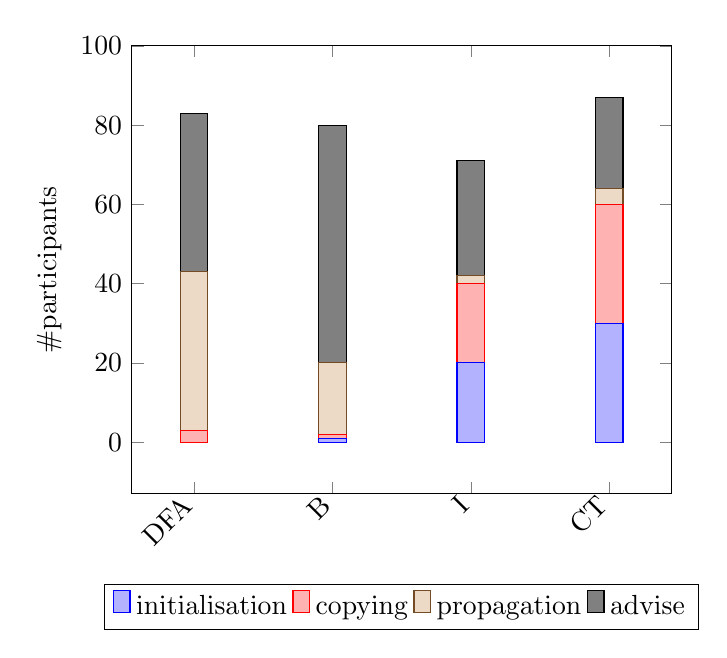
\begin{tikzpicture}
\begin{axis}[
    ybar stacked,
    enlargelimits=0.15,
    legend style={at={(0.5,-0.20)},
      anchor=north,legend columns=-1},
    ylabel={\#participants},
    symbolic x coords={DFA,B,I,CT},
    xtick=data,
    x tick label style={rotate=45,anchor=east},
    ]

    \addplot+[ybar] plot coordinates 
    {(DFA,0) (B,1) (I,20) (CT,30)};
    \addplot+[ybar] plot coordinates 
    {(DFA,3) (B,1) (I,20) (CT,30)};
    \addplot+[ybar] plot coordinates 
    {(DFA,40) (B,18) (I,2) (CT,4)};
    \addplot+[ybar] plot coordinates 
    {(DFA,40) (B,60) (I,29) (CT,23)};
    
    

% \addplot+[ybar] plot coordinates {(tool1,0) (tool2,2) 
%   (tool3,2) (tool4,3) (tool5,0) (tool6,2) (tool7,0)};

% \addplot+[ybar] plot coordinates {(tool1,0) (tool2,0) 
%   (tool3,0) (tool4,3) (tool5,1) (tool6,1) (tool7,0)};

% \addplot+[ybar] plot coordinates {(tool1,6) (tool2,6)
%   (tool3,8) (tool4,2) (tool5,6) (tool6,5) (tool7,6)};

% \addplot+[ybar] plot coordinates {(tool1,4) (tool2,2) 
%   (tool3,0) (tool4,2) (tool5,3) (tool6,2) (tool7,4)};

    \legend{initialisation,copying,propagation,advise}
\end{axis}
\end{tikzpicture}